% !TeX spellcheck = en_US
% !TeX encoding = UTF-8
\documentclass[11pt, a4paper]{article}
\usepackage{graphics, graphicx}
\usepackage{fancyvrb, enumerate}
\usepackage{amsmath, amssymb, amscd, amsfonts}
\usepackage{geometry}
\usepackage{multirow}
\usepackage{url}
\usepackage{tikz}
\usepackage{listings, listing}
\usepackage{color}
\usepackage{mathptmx}
\usepackage{apacite}
\usepackage[style=iso]{datetime2}

\usetikzlibrary{shapes, arrows, calc, positioning}
\definecolor{codegreen}{rgb}{0, 0.6, 0}
\definecolor{codegray}{rgb}{0.5, 0.5, 0.5}
\definecolor{codepurple}{rgb}{0.58, 0, 0.82}
\definecolor{backcolour}{rgb}{0.95, 0.95, 0.92}
\lstdefinestyle{mystyle}
{
    backgroundcolor=\color{backcolor},
    commentstyle=\color{codegreen},
    keywordstyle=\color{magenta},
    numberstyle=\tiny\color{codegray},
    stringstyle=\color{codepurple},
    basicstyle=\footnotesize,
    breakatwhitespace=false,
    breaklines=true,
    captionpos=b,
    keepspaces=true,
    numbers=left,
    numbersep=5pt,
    showspaces=false,
    showstringspaces=false,
    showtabs=false,
    tabsize=2,
    frame=single
}
\lstset{style=mystyle}
\tikzstyle{decision} = [diamond, draw, fill=blue!20, text width=4.5em, text badly centered, node distance=3cm, inner sep=0pt]
\tikzstyle{block} = [rectangle, draw, fill=blue!20, text width=5em, text centered, rounded corners, minimum height=2em]
\tikzstyle{line} = [draw, -latex']
\tikzstyle{cloud} = [draw, ellipse, fill=red!20, node distance=5em, minimum height=2em]
\tikzset
{
    -|-/.style=
    {
        to path=
        {
            (\tikztostart) -| ($(\tikztostart)!#1!(\tikztotarget)$) |- (\tikztotarget)
            \tikztonodes
        }
    },
    -|-/.default=0.5,
    |-|/.style=
    {
        to path=
        {
            (\tikztostart) |- ($(\tikztostart)!#1!(\tikztotarget)$) -| (\tikztotarget)
            \tikztonodes
        }
    },
    |-|/.default=0.5,
}

\geometry
{
    top = 20mm,
    bottom = 20mm,
    left = 20mm,
    right = 20mm
}

\title{Helixco Cavity}
\author{Jaewoong Lee}
\date{\today}

\begin{document}
    \maketitle
    \newpage

    \tableofcontents
    \listoftables
    \listoffigures
    \newpage

    \section{Introduction}
        \subsection{Dental Cavity}
            Dental cavity is one of the most common bacterial infections in humans. \textit{Streptococcus mutans} in the acquired enamel pellicle have a main role in human dental cavity \cite{cavity1, cavity2}.

            \begin{figure}[htbp]
                \centering
                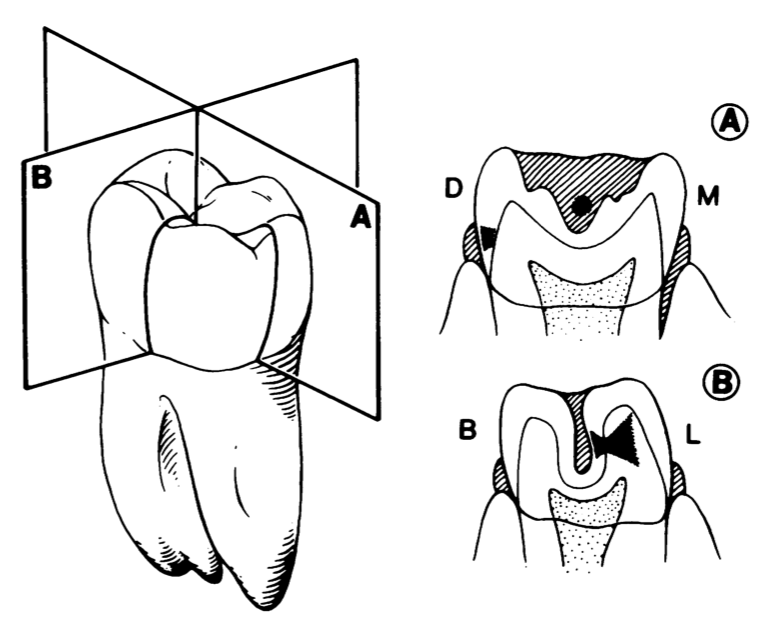
\includegraphics[width=0.4 \linewidth]{figures/molar.png}
                \caption{Saggital and cross-sectional sections through a permanent molar \protect \cite{cavity1}}
                \label{fig:molar}
            \end{figure}

        \subsection{Microbiome}

    \section{Materials}
        \subsection{Microbiome analysis}

    \section{Methods}
        \subsection{Docker}
            Docker is light-weight linux containers for consistent development and deployment \cite{docker1}.

        \subsection{QIIME 2}
            QIIME 2 is a powerful, extensible, and decentralized microbiome analysis package with a focus on data and analysis transparency.

        \subsection{Scikit-learn}
            Scikit-learn is a simple and efficient tools for predictive data analysis \cite{sklearn1, sklearn2}.

    \section{Results}

    \section{Discussion}

    \bibliographystyle{apacite}
    \bibliography{reference}
\end{document}